\documentclass[sigconf]{acmart}
\title{Simulation von Protuberanzen und Erstellen von prozeduralen Kugeloberflächen in Unity}
\author{Florian Hansen}

\affiliation{
  \institution{Hochschule Flensburg}
}

\usepackage[ngerman]{babel}

\settopmatter{printacmref=false}
\renewcommand\footnotetextcopyrightpermission[1]{}
\pagestyle{plain}

\begin{document}
  \begin{abstract}
    test
  \end{abstract}
  \maketitle

  \section{Einleitung}
Häufig steht man als 3D-Programmierer vor dem Problem, die in der Natur
vorkommenden Phänomene effizient und in Echtzeit darzustellen zu wollen, um
diese dann anschließend in andere Projekte wie Videospiele einzubinden. Aber
auch bei Filmen sollte darauf geachtet werden, dass die Zeit für das Rendern
nicht ausartet. Am interessantesten erscheint in diesem Zusammenhand die Nutzung
von Echtzeitsimulationen, um natürliche Prozesse näher untersuchen zu können,
die nicht so häufig vorkommen.

Im Grunde existieren zwei Lösungsansätze für das Problem, rechenintensive
Echtzeitsimulationen durchzuführen. Zum einen kann man fiktive Effekte
definieren, die durch iteratives Ausprobieren ähnliche Ergebnisse wie das reale
Vorbild erzielen. Diese Ergebnisse sind dann jedoch rein fiktiv und haben selten
etwas mit der Realität zu tun. Zum anderen kann man versuchen, physikalische
Prozesse abzubilden, um so möglichst nah an der Realität zu bleiben. Diese
wissenschaftliche Arbeit soll sich diesem Problem anhand der uns bekannten Sonne
widmen. Hierbei wird sich auf die äußerliche Erscheinung der Sonne und besonders
ihrer Protuberanzen (umgangssprachlich Sonnenstürme) bezogen. Es soll also eine
Verbindung zwischen echten, beobachtbaren Phänomenen bzw.  physikalischen
Eigenschaften der Sonne und Computersimulationen umgesetzt werden.

  \section{Grundlagen}
\subsection{GLSL-Shader}
\subsection{HLSL-Shader}
\subsection{CG-Shader}
  \section{Berechnung einer Kugel}
Damit später eine Textur für die Sonne erstellt werden kann, muss zuerst eine
Oberfläche generiert werden, die diese Textur aufnehmen kann. Hierfür existieren
verschiedenste Möglichkeiten. Im Falle der Sonne betrachten wir das Modell einer
Kugel, die später manipuliert werden soll, um visuelle Effekte auf ihr
abzubilden. Beim Betrachten der folgenden Algorithmen zur Erzeugung von
Kugeloberflächen wird klar, dass nicht alle Methoden für dieses Vorhaben
geeignet sind. Aus diesem Grund werden die einzelnen Verfahren näher erläutert
und anschließend abgewogen, welcher Algorithmus zur Erzeugung einer
Sonnenoberfläche verwendet werden sollte.

\subsection{Längengrad-Breitengrad-Gitter}
Die einfachste Möglichkeit, eine Kugeloberfläche zu erzeugen, ist die Verwendung
von Segmentlinien. Im Grunde unterteilt man die gesamte Kugel in Schichten,
deren Umfang schließlich die Oberfläche der Kugel darstellen. Die Mesh-Punkte
(\textit{Vertices}) dieser Schichten, welche als einfache Kreise wahrgenommen
werden können, werden mithilfe von Längen- und Breitengradinformationen
erstellt. Das Resultat ist eine Kugeloberfläche mit erkennbaren Polen an der
Ober- und Unterseite der Oberfläche. Diese entstehen dadurch, dass auch am Rand
der Kugel die gleiche Anzahl an Kanten vorhanden ist, wie am Äquator. Diese
Schichten sind dementsprechend lediglich herunterskaliert und in einem immer
kürzer werdenden Abstand aufeinander geschichtet und Erzeugen eine Überabtastung
am oberen und unteren Rand der Kugel \cite{Gonzalez2009}.

Die Überabtastung an den Polen bzw. die Unterabtastung am Äquator bringt viele
Probleme mit sich. Vor allem, wenn die Oberfläche animiert werden soll,
erscheint die Animation als sehr unregelmäßig. Hierauf wird jedoch in einem
späteren Abschnitt eingegangen, wenn die hier vorgestellten Methoden miteinander
verglichen werden.

\subsection{Fibonacci-Gitter}
Um das Problem der Inhomogenität von Längengrad-Breitengrad-Gittern zu lösen,
können Fibonacci-Gitter verwendet werden. Hierbei werden die Punkte des Gitters
entlang einer Spirale, die sogenannte Fibonacci-Spirale, angeordnet. Wichtig bei
der Konstruktion sind die \textit{Golden-Ratio} $\Phi$ und der
\textit{Golden-Angle} $\alpha$ \cite{Gonzalez2009, Marques2013}.

$$\Phi = \frac{1 + \sqrt{5}}{2} \quad\quad\quad \alpha = 2\pi\left(2 - \Phi\right)$$

Besonders einfach lässt sich bei diesem Algorithmus die Anzahl an Oberflächenpunkte
kontrollieren. Das folgende Beispiel behandelt das Erstellen von $N$ Punkten,
die gleichmäßig verteilt auf der Oberfläche einer Kugel liegen. Zuerst werden
die Längen- und Breitengrade der einzelnen Punkte berechnet.

$$lat_i = arcsin\left(\frac{2i}{N + 1} - 1\right) \quad\quad\quad
lon_i = \alpha \cdot i$$

Anschließend können die räumlichen Koordinaten als Positionsvektor $\vec{p} \in
\mathbb{R}^3$ wie folgt berechnet werden.

\[
\vec{p} =
\left(\begin{array}{c}
    \cos\left(lon\right) cos\left(lat\right) \\
    \sin\left(lon\right) sin\left(lat\right) \\
    \sin\left(lat\right)
\end{array}\right)
\]

Wie man sieht, ist die Erzeugung von homogen verteilten Oberflächenpunkten einer
Kugel mithilfe von Fibonacci-Gittern ziemlich schnell implementiert. Nachteil
dieser Lösung ist, dass lediglich die Punkte bzw. Vertices eines Meshes erzeugt
werden. Um Flächen darstellen zu können, muss nachträglich eine Triangulation
stattfinden. 

\subsection{Ikosaeder}
Genau wie das Fibonacci-Gitter erzeugt ein Ikosaeder gleichmäßig verteilte
Punkte auf der Oberfläche einer Kugel. Das Verfahren ist trotzdem komplett
unterschiedlich. Anstatt die Vertices des Meshes zu berechnen und
anschließend diese miteinander in Dreiecke zu verbinden, wird eine initiale
Geometry erzeugt, dessen Flächen wiederum in weitere Flächen unterteilt wird.
Dieses Vorgehen wird beliebige Male wiederholt, um eine immer glattere
Oberfläche zu erzeugen. Das Problem bei diesem Algorithmus ist, dass durch
die Unterteilung der Flächen in weitere, kleinere Flächen auf den ersten
Blick nicht abgeschätzt werden kann, wie viele Vertices genau berechnet
werden müssen. Tabelle \ref{table:icosahedron-complexity} zeigt den Anstieg
der benötigten Punkte, die durch $N$ wiederholten Unterteilungsschritten
berechnet werden müssen. Anhand der Anzahl an Dreiecken fällt ein
exponentielles Wachstum auf, weshalb eine Erhöhung der
Unterteilungsiterationen mit Bedacht durchgeführt werden sollte. Eine kleine
Veränderung von $N$ hat große Auswirkung auf die benötigte Rechenleistung für
das Kugelmesh.

\begin{table}
  \caption{Vergleich zwischen Anzahl der Unterteilungsiterationen $N$ und den erzeugten neuen Flächen bzw. Vertices}
  \label{table:icosahedron-complexity}
  \begin{tabularx}{\columnwidth}{lXX}
    \textbf{N} & \textbf{Anzahl Vertices} & \textbf{Anzahl Dreiecke} \\
    \hline
    1 & 12   & 60 \\
    2 & 42   & 240 \\
    3 & 162  & 960 \\
    4 & 642  & 3840 \\
    5 & 2562 & 15360
  \end{tabularx}
\end{table}


\subsection{Entwicklung eines Skripts}

  \section{Sonnenoberfläche}
In diesem Abschnitt wird besprochen, wie die Sonnenoberfläche in der Realität
aussieht und wie die Erscheinung prodedural Nachgebildet werden kann. Dabei
wird insbesondere auf die Entwicklung eines entsprechenden CG-Shaders
eingengangen. Grundsätzlich besteht die Möglichkeit, eine Textur zu
generieren, diese in eine Datei zu speichern und anschließend auf das Mesh zu
übertragen. Dies hat jedoch den Nachteil, dass die Textur nur unter sehr
hohem Aufwand über die Zeit verändert werden kann. Deshalb soll die
Oberflächentextur im Shader selbst erzeugt werden, sodass diese in Echtzeit
animiert werden kann. Auch wird das Verfahren erläutert, wie die
Sonnengeometrie erzeugt wird und für den Shader vorbereitet wird.

\subsection{Generierung der Geometrie} 
Bevor eine Textur für die Sonne dargestellt werden kann, müssen zuerst alle
Rahmenbedingungen stimmen. Dies beinhaltet vor allem die Vorbereitung eines
geeigneten Meshes für die Sonnenoberfläche. Im Folgenden wird der Algorithmus
vorgestellt, welcher eine homogene Geometrie für die Sonne erstellt. Dieser
erstellt in erster Linie die Eckpunkte einer Icosphere. Eine Icosphere
besitzt 20 Dreiecke bestehend aus 12 Eckpunkten, welche die Grundlage für
weitere Unterteilungsschritte sind. Dementspreched müssen diese initial
berechnet werden. Anschließend startet der eigentliche Algorithmus zum
Unterteilen der Flächen in kleinere Flächen. Dieser berechnet auf jeder Kante
eines Dreiecks einen Mittelpunkt, sodass für jede Dreiecksfläche insgesamt
drei neue Eckpunkte entstehen. Anschließend müssen die neu erzeugten Punkte
auf die Einheitskugel abgebildet werden, indem die Positionsvektoren
normalisiert werden. Algorithmus \ref{alg:icosphere} soll diesen Vorgang
verdeutlichen.

\begin{algorithm}
  \caption{Unterteilen von Dreiecksflächen auf einer Icosphere}
  \label{alg:icosphere}
  \SetAlgoLined

  \SetKwInOut{Input}{Eingabe}\SetKwInOut{Output}{Ausgabe}

  \Input{Flächen des Basismeshes $M$, Rekursionslevel $n$}
  \Output{Mesh einer Icosphere mit unterteilten Flächen}
  \BlankLine
  \For{$i\leftarrow 0$ \KwTo $n$}{
    $M'\leftarrow \{\}$\;
    \BlankLine
    \ForEach{$d \in M$}{
      $(\vec{a},\;\vec{b},\;\vec{c})\leftarrow d$\;
      \BlankLine
      $\vec{a}'\leftarrow$ calculateMiddlePoint($\vec{a}$, $\vec{b}$)\;
      $\vec{b}'\leftarrow$ calculateMiddlePoint($\vec{b}$, $\vec{c}$)\;
      $\vec{c}'\leftarrow$ calculateMiddlePoint($\vec{c}$, $\vec{a}$)\;
      \BlankLine
      append($M'$, $(\vec{a},\;\vec{a}',\;\vec{c}')$)\;
      append($M'$, $(\vec{b},\;\vec{b}',\;\vec{a}')$)\;
      append($M'$, $(\vec{c},\;\vec{c}',\;\vec{b}')$)\;
      append($M'$, $(\vec{a}',\;\vec{b}',\;\vec{c}')$)\;
    }
    \BlankLine
    $M\leftarrow M'$\;
  }
\end{algorithm}

\begin{figure}
  
\includegraphics[width=\columnwidth]{icosphere-algorithm}
  \caption{Vergleich zwischen unterschiedlichen Rekursionslevel von Algorithmus \ref{alg:icosphere}. Links befindet sich das Basismodell, in der Mitte die erste und rechts die zweite Rekursionsstufe.}
  \label{fig:icosphere-levels}
  \Description[]{}
\end{figure}

\subsection{Fractal Brownian Motion}
Eine Textur zu erzeugen, die zu jeden Zeitpunkt gleich aussieht wirkt oft
langweilig und uninteressant. Auch, wenn man das Vorbild dieser Arbeit
betrachtet -- die Sonne --, unterscheidet sich die Oberfläche zu jedem
Zeitpunkt von einer vorherigen Messung. Um ein solchen Phänomen zu
modellieren, bedient man sich häufig dem Rauschen. Rauschen hat für
unterschiedliche Fachgebiete eine unterschiedliche Bedeutung. Musiker
verbinden damit störende Geräusche und Astrophysiker denken dabei an
kosmische Hintergrundstrahlung \cite{bookofshaders}. In der Computergrafik
versucht man hingegen, dieses Rauschen künstlich zu generieren, um
beispielsweise eine Textur prozedural zu erzeugen. Auch in dieser Arbeit soll
die Oberflächentextur der Sonne durch ein künstliches Rauschen erzeugt und
verändert werden. Dies entspricht natürlich nicht der Realität, denn die
Sonnenoberfläche hängt von vielen Faktoren, wie der Temperatur und dem
Magnetfeld der Sonne ab. Auch kann man sogenannte Sonnenflecken beobachten,
welche sich als dunkle Flecken auf der Oberfläche äußern. Diese sind nicht
wirklich schwarz, sondern erscheinen dunkler als ihre Umgebung, da diese
Stellen niedrigere Temperaturen aufweisen.

Anstatt nun zu versuchen, die Oberfläche der Sonne so realitätsgetreu wie
möglich nachzubilden, wird in diesem Projekt versucht, mithilfe von künstlich
erzeugtem Rauschen eine ähnliche Oberfläche zu generieren. Hierfür wird, wie
der Titel des Abschnitts andeutet, \textit{Fractal Brownian Motion} (fBM) verwendet.
Oft werden hierbei Begriffe wie \textit{Oktaven}, \textit{Porosität} und
\textit{Zuwachs} genannt. Eine Oktave beschreibt eine Summe aus mehreren
Rauschfunktionen, die Porosität die Multiplikation der Frequenz um einen konstanten
Wert und der Zuwachs die Verringerung der Amplitude. Algorithmus \ref{alg:fbm} zeigt
ein einfaches zweidimensionales frakturiertes Rauschen basierend auf \cite{bookofshaders}.

\begin{algorithm}
  \caption{Fractal Brownian Motion mit eindimensionaler Eingabe}
  \label{alg:fbm}
  \SetAlgoLined

  \SetKwInOut{Input}{Eingabe}\SetKwInOut{Output}{Ausgabe}

  \Input{$x \in \mathbb{R}$, $\mathit{octaves} \in \mathbb{N}$}
  \Output{$y \in \mathbb{R}$}
  \BlankLine
  $y \leftarrow 0$\;
  $\mathit{lacunarity}\leftarrow 2$\;
  $\mathit{gain}\leftarrow 0.5$\;
  \BlankLine
  $\mathit{amplitude}\leftarrow 0.5$\;
  $\mathit{frequency}\leftarrow 1$\;
  \BlankLine
  \For{$i\leftarrow 0$ \KwTo $\mathit{octaves}$}{
    $y = y + \mathit{amplitude} * \mathit{noise}(\mathit{frequency} \cdot x)$\;
    $\mathit{frequency} = \mathit{frequency} \cdot \mathit{lacunarity}$\;
    $\mathit{amplitude} = \mathit{amplitude} \cdot \mathit{gain}$\;
  }
  \BlankLine
  \Return y\;

\end{algorithm}

Die Abbildung zum Erzeugen von Rauschen (\textit{noise}) kann dabei beliebig
gewählt werden. In den meisten Fällen erzeugt man jedoch kein echtes Rauschen,
welches eine nicht stetische Funktion darstellen würde. Stattdessen wird
mithilfe von überlagerten Wellenfunktionen künstliches stetiges Rauschen
implementiert. Dies hat den Vorteil, dass sich das Rauschverhalten periodisch
ist, d.h. dass sich die Werte abhängig von der Zeit irgendwann wiederholen. Dies
ist unter anderem daher sinnvoll, da im Falle einer Textur sonst Sprünge bzw.
harte Kanten erzeugt werden. Um fBM nun in der Textur verwenden zu können muss
die Funktion \textit{noise} näher betrachtet werden. Im Algorithmus
\ref{alg:fbm} wird die Abbildung $\text{noise}: \mathbb{R} \to \mathbb{R}$
verwendet. Als Eingabe wird also eine reelle Zahl genommen und auf eine andere
reelle Zahl abgebildet. Um nun eine Textur zu erzeugen muss beachtet werden,
dass das Mesh, dessen Oberfläche mit der Textur ausgestattet werden soll,
sogenannte UV-Koordinaten pro Eckpunkt definiert. Anhand dieser UV-Koordinaten
wird dann die entsprechende Stelle in der Textur verwendet und auf den Eckpunkt
projeziert. Da eine Textur häufig zweidimensional ist, sind die UV-Koordinaten
ebenfalls zweidimensionale Angaben. Die Abbildung muss nun also umgewandelt
werden, sodass $\text{noise}: \mathbb{R}^2 \to \mathbb{R}$ gilt. Es ändert sich
am Algorithmus selbst jedoch nichts, außer dass als Eingabe UV-Koordinaten
$\in \mathbb{R}^2$ genommen werden, anstatt eine Ganzzahl $\in \mathbb{R}$.
Jedoch muss dadurch ebenfalls die \textit{noise}-Funktion von einem 2D-Vektor
abhängen. Algorithmus \ref{alg:2d-noise} und \ref{alg:2d-hash} zeigen
Beispielimplementationen dieser Funktionen. Damit wird bei einer
Eingabe eines zweidimensionalen Vektors eine reelle Zahl abgebiltet, die im
darauf folgenden Schritt als Farbwert verwendet werden kann. Mit anderen
Worten, der Algorithmus \ref{alg:suntexture} liefert dann zu jeder UV-Koordinate einen
entsprechenden Graustufenwert der Textur.

\begin{algorithm}
  \caption{Beispiel für die Hashfunktion \textit{hash} mit einer zweidimensionalen Eingabe.}
  \label{alg:2d-hash}
  \SetKwInOut{Input}{Eingabe}\SetKwInOut{Output}{Ausgabe}
  \SetAlgoLined

  \Input{$\vec{n} \in \mathbb{R}^2$}
  \Output{$h \in \mathbb{R}$}
  \BlankLine
  $a\leftarrow 123.456789$\;
  $b\leftarrow 987.654321$\;
  $c\leftarrow 54321.9876$\;
  \BlankLine
  $s\leftarrow \sin(\operatorname{dot}(\vec{n}, (a, b)^T))$\;
  $h\leftarrow \operatorname{frac}(s \cdot c)$\;
  \BlankLine
  \Return $h$\;
\end{algorithm}

\begin{algorithm}
  \caption{Beispiel für die Rauschfunktion \textit{noise} mit einer zweidimensionalen Eingabe.}
  \label{alg:2d-noise}
  \SetKwInOut{Input}{Eingabe}\SetKwInOut{Output}{Ausgabe}
  \SetAlgoLined

  \Input{$\vec{p} \in \mathbb{R}^2$}
  \Output{$r \in \mathbb{R}$}
  \BlankLine
  $\vec{i}\leftarrow \operatorname{floor}(\vec{p}) \in \mathbb{R}^2$\;
  $\vec{u}\leftarrow \operatorname{smoothstep}(0, 1, \operatorname{frac}(\vec{p})) \in \mathbb{R}^2$\;
  $a\leftarrow \operatorname{hash}(i + (0, 0)^T)$\;
  $b\leftarrow \operatorname{hash}(i + (1, 0)^T)$\;
  $c\leftarrow \operatorname{hash}(i + (0, 1)^T)$\;
  $d\leftarrow \operatorname{hash}(i + (1, 1)^T)$\;
  $r\leftarrow \operatorname{lerp}(\operatorname{lerp}(a, b, x_u), \operatorname{lerp}(c, d, x_u), y_u)$\;
  \BlankLine
  \Return $r^2$\;
\end{algorithm}

\begin{algorithm}
  \caption{Erzeugen der Sonnentextur unter der Verwendung von Fractal Brownian
  Motion}
  \label{alg:suntexture}
  \SetKwInOut{Input}{Eingabe}\SetKwInOut{Output}{Ausgabe}
  \SetAlgoLined

  \Input{UV-Koordinate $\mathit{uv}$, Anzahl der Oktaven $n$}
  \Output{Farbvektor $\vec{c}$}
  \BlankLine
  $y_\mathit{fbm} \leftarrow \operatorname{fbm}(\mathit{uv} +
    \operatorname{fbm}(\mathit{uv}, n), n)$\;
  $\vec{c} \leftarrow (y_\mathit{fbm}, y_\mathit{fbm}, y_\mathit{fbm})$\;
  \Return $\vec{c}$\;
\end{algorithm}

\begin{figure}
  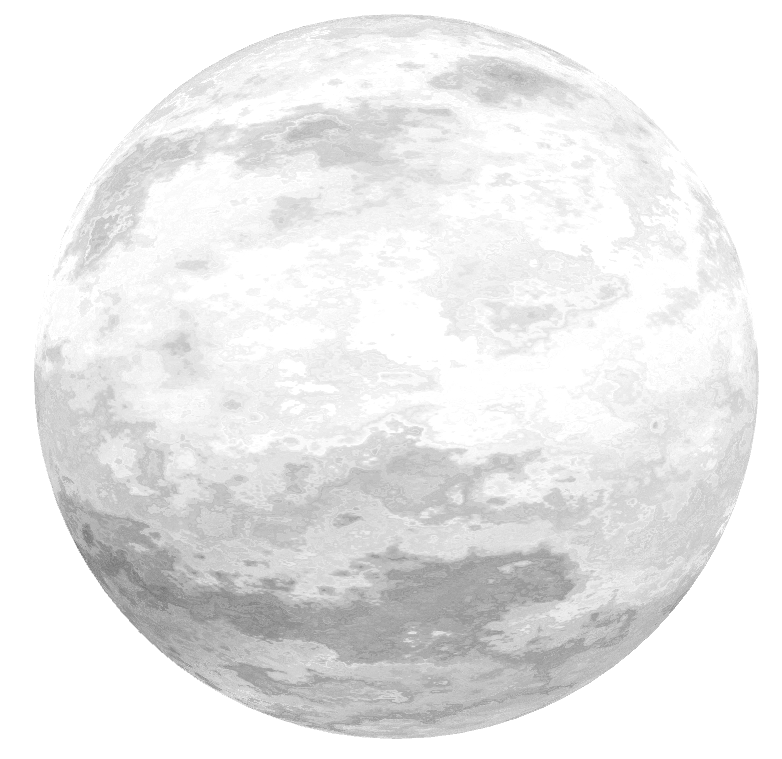
\includegraphics[width=0.6\columnwidth]{fbm-sphere}
  \caption{Anwendung von fBM auf einer Icosphere mit einer Amplitude von 0.86, einer Porosität von 4.56 und einem Zuwachs von 0.55.}
  \Description[fBM auf Icosphere]{Anwendung von fBM auf einer Icosphere mit einer Amplitude von 0.86, einer Porosität von 4.56 und einem Zuwachs von 0.55.}
\end{figure}
  \section{Protuberanzen}
\subsection{Wie Sonnenstürme entstehen}
\subsection{Magnetische Felder am Beispiel eines Dipols}
\subsection{Erstellung eines Vektorenfelds}
\subsection{Aufbau eines Partikelsystems}

  \section{Fazit und Ausblick}


  \bibliography{literature}
  \bibliographystyle{abbrv}
\end{document}
